\documentclass[12pt,titlepage]{article}

%% THE USEPACKAGES NECESSARY FOR THIS EXAMPLE
%% NOTE THAT genetics_manu_style MUST BE CALLED AFTER mychicago
\usepackage{graphicx}
%\usepackage{figcaps}
\usepackage[nomarkers,notablist,nofiglist,tablesfirst]{endfloat}
\usepackage{amsfonts}
\usepackage{sectsty}
%\usepackage{subfigure}
%\usepackage{subcaption}
\usepackage{natbib} \bibpunct{(}{)}{;}{author-year}{}{,} 
\usepackage[usenames,dvipsnames,svgnames,table]{xcolor}
%\allsectionsfont{\sffamily}
%% THE MANUSCRIPT TITLE

\usepackage{caption}
\usepackage[labelformat=simple]{subcaption}

\usepackage{bibentry}

\usepackage{xr}
\externaldocument{hybrid_zone}

\newcommand{\alisa}[1]{{\em \color{red} #1}}
\newcommand{\plr}[1]{{\em \color{blue} #1}}
\newcommand{\yb}[1]{{\em \color{magenta} #1}}


\newcommand{\given}{\,\vert\,}
\newcommand{\st}{\,\colon\,}
\renewcommand{\and}{\,\&\,}


\begin{document}
\setcounter{table}{0}
\renewcommand{\thetable}{S\arabic{table}}
\setcounter{figure}{0}
\renewcommand{\thefigure}{S\arabic{figure}}

\begin{figure}
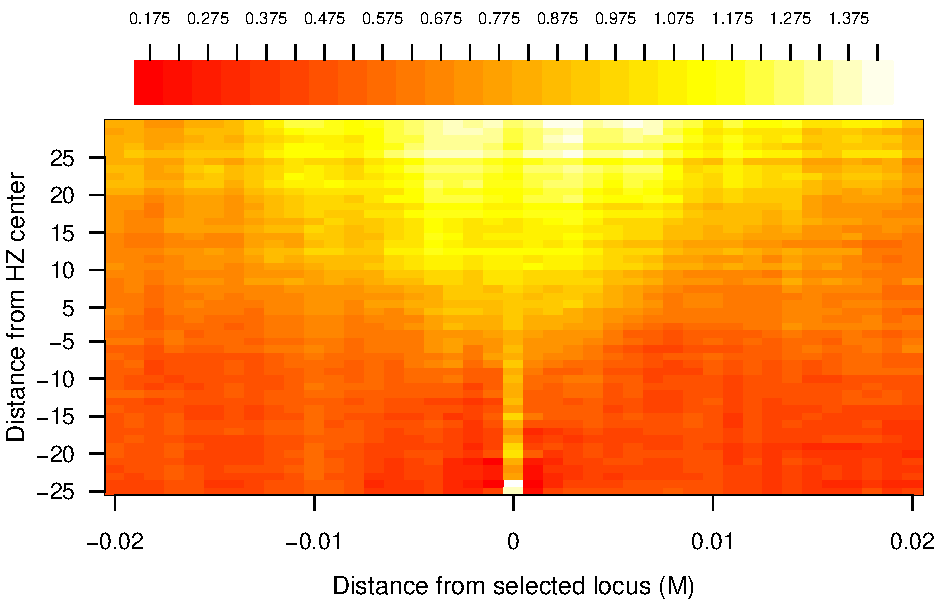
\includegraphics{figs/blocksAlongChromHeatmapAncBConditioning}
\caption{Heatmap of mean block length $l_B(m_i)$ along a simulated chromosome. }\label{Supp:blockLengthHeatmap}
\end{figure}



\begin{figure}
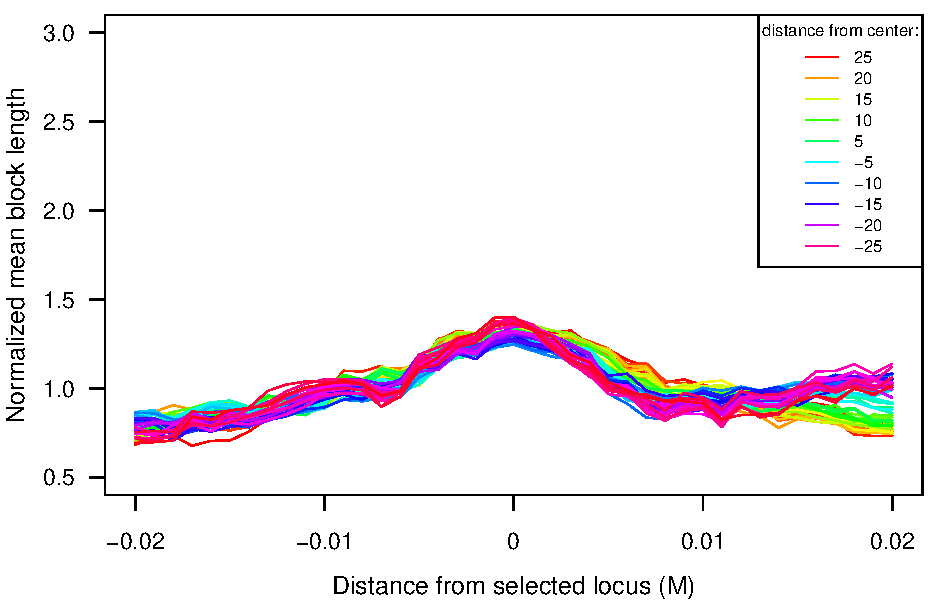
\includegraphics{figs/blocksAlongChromNoConditioning}
\caption{Heatmap of mean block length $l_\bullet(m_i)$ surrounding a given position along the genome with a single underdominant site ($s=0.01, \tau=1000$). }\label{Supp:blockLengthNoAnc}
\end{figure}

\begin{figure}
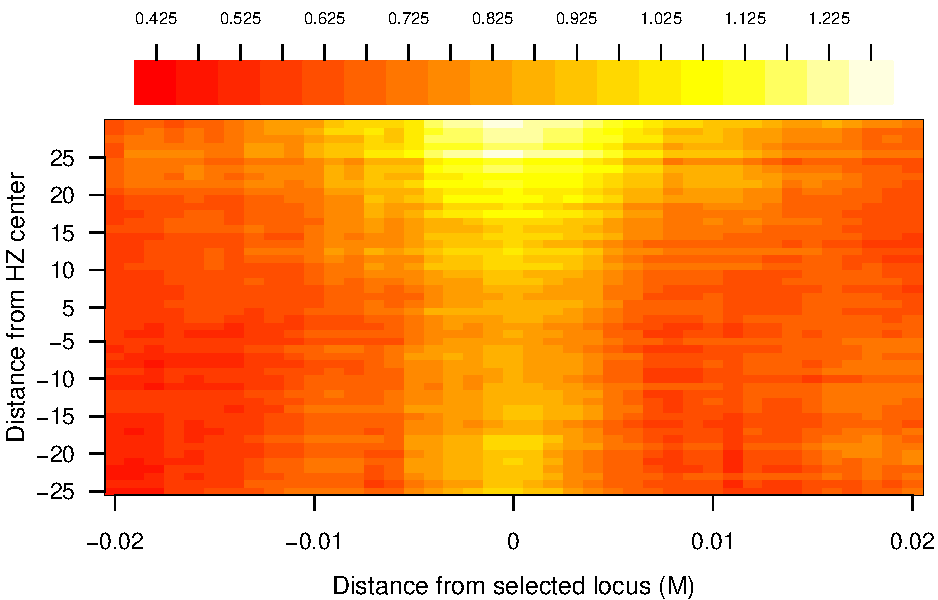
\includegraphics{figs/blocksAlongChromHeatmap}
\caption{Heatmap of mean block length $l_\bullet(m_i)$ along a simulated chromosome with a single underdominant site ($s=0.01, \tau=1000$) }\label{Supp:blockLengthHeatmapNoAnc}
\end{figure}


\begin{figure}
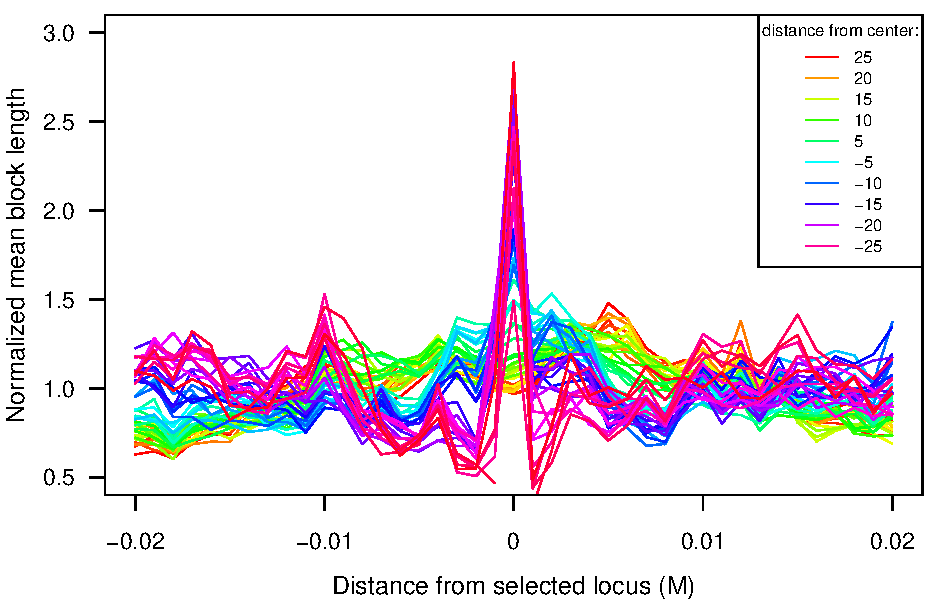
\includegraphics{figs/ratioAdjacentBlocksAlongChromAncBConditioning}
\caption{Ratio $\frac{2\sum{l_B(m_i)}}{\sum{l_A(m_i-)+I_A(m_i+)}}$ of mean block length and adjacent block lengths across a simulated chromosome with a single underdominant site ($s=0.01, \tau=1000$).  Each line represents a deme and is normalized by mean block length across the chromosome in the deme.}\label{Supp:ratioBlockAdjacent}
\end{figure}


\begin{figure}
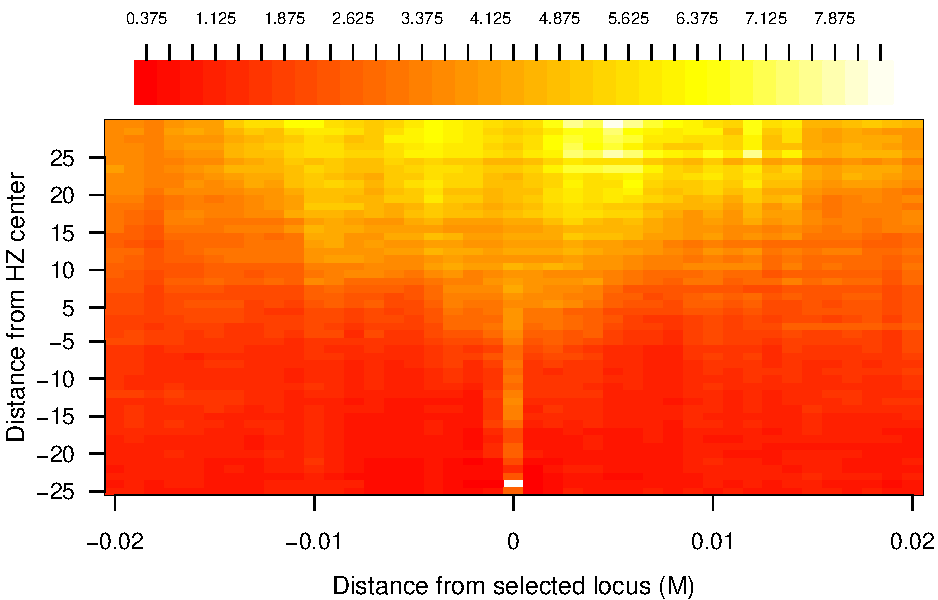
\includegraphics{figs/ratioAdjacentBlocksAlongChromHeatmapAncBConditioning}
\caption{Heatmap of $\frac{2\sum{l_B(m_i)}}{\sum{l_A(m_i-)+I_A(m_i+)}}$ across a simulated chromosome with a single underdominant site ($s=0.01, \tau=1000$). }\label{Supp:ratioBlockAdjacentHeatmap}
\end{figure}


\end{document}